\documentclass{article}

\usepackage{amsmath}
\usepackage{parskip}
\usepackage{listings}
\usepackage[table]{xcolor}
\usepackage{tikz}
\def\checkmark{\tikz\fill[scale=0.4](0,.35) -- (.25,0) -- (1,.7) -- (.25,.15) -- cycle;}
\usepackage{graphicx}
\usepackage{subfig}
\usepackage{floatrow}

\graphicspath{{./}} 

\lstset{
  basicstyle=\ttfamily\scriptsize
}

\begin{document}

\title{COMN Study Helper}
\date{}
\maketitle
\pagestyle{empty}

\section{COMN Basics}
\subsection{General Definitions}

\textbf{Bandwidth}
The maximum transfer rate over some link.

\textbf{Throughput}
The rate of \textit{successful} data transfer over some channel.

\textbf{Delay}
The time it takes from one portion of data to go between two nodes.

\textit{sources of packet delay}:

\fbox{
  \parbox{\textwidth}{
    \textbf{Nodal Processing}:\\

    Time taken by a node to process the information it receives, usually negligible.\\

    \textbf{Queuing Delay}:\\

    Time spent waiting at a link to be transmitted.\\

    $\frac{\text{Packet Length}\times\text{Average Packet Arrival Rate}}{\text{Link Bandwidth}}$\\

    \textbf{Transmission Delay}:\\

    $\frac{\text{Packet length}}{\text{Link Bandwidth}}$\\

    \textbf{Propagation Delay}:\\

    $\frac{\text{Length of Physical Link}}{\text{Propagation Speed in Medium}}$

  }
}

\textbf{Packet Loss}

When a packet has been lost, or dropped. This can happen when the buffer at a link is full and is unable to pass it on.

\textbf{BDP: Bandwidth-Delay Product}

$\text{Link Bandwidth}\times\text{Round-Trip Delay Time}$

Tells us the maximum amount of data that may be on a circuit at any one time, that is data that has been transferred but not yet acknowledged.

\textbf{Packet Sniffing}

When a network interfaces records all packets that 'pass by' it.

\textbf{IP Spoofing}

Sending data packets that have \textit{forged} source addresses on them.

\textbf{Layering}

Network systems are broken into layers, to allow for the identification and relationship between each piece in a network. Makes troubleshooting easier. There are two versions, the \textit{Internet Protocol Stack} and the \textit{OSI Model}, which are very similar.

\begin{figure}[h]

  \begin{floatrow}
  \subfloat[IP Stack]{
    \begin{tabular}{|c|c|}
      \hline
      5 & Application\\
      \hline
      4 & Transport\\
      \hline
      3 & Network\\
      \hline
      2 & Link\\
      \hline
      1 & Physical\\
      \hline
    \end{tabular}
  }

  \quad

  \subfloat[OSI Model]{
    \begin{tabular}{|c|c|}
      \hline
      7 & Application\\
      \hline
      6 & Presentation\\
      \hline
      5 & Session\\
      \hline
      4 & Transport\\
      \hline
      3 & Network\\
      \hline
      2 & Data Link\\
      \hline
      1 & Physical\\
      \hline
    \end{tabular}
  }
  \end{floatrow}
\end{figure}

\textbf{Encapsulation}

The logical separation of modular layers, utilised by both the OSI Model and the IP Stack. These can be inspected when looking at the headers of that data that is transferred over the network. Most layers will add header information that is required for them to work properly.

These are called \textit{Protocol Data Units}, when browsing a website, the payload may be \textit{encapsulated} within TCP, IP and frame (Data Link layer) headers.

\fbox{
  \parbox{\textwidth}{

    \textbf{\underline{OSI Model/IP Stack Breakdown}}\\

    \textbf{Application}\\

    Annoyingly has two different definitions under the IP stack and OSI model.

    \textit{OSI Definition}:\\

    High-level APIs.\\

    \textit{IP Stack Definition}:\\

    Supports network layer applications, e.g. HTTP, FTP.\\

    \textbf{Presentation}\\

    \textit{OSI Only.}\\
    
    Translation between application and network layers, e.g. HTML, CSS\\

    \textbf{Session}\\

    \textit{OSI Only.}\\

    Management of continuous communications or sessions between two nodes, e.g. HTTP, FTP.\\

    \textbf{Transport}\\

    Makes use of \underline{segments (TCP) or datagrams (UDP)}.\\

    Transmission of data segments between two nodes, e.g. UDP, TCP.\\

    \textbf{Network}\\
    
    Makes use of \underline{packets}.\\

    Routing of datagrams between source and destination, e.g. IPv4, IPv6.\\
    
    \textbf{Link/Data Link}\\

    Makes use of \underline{frames}.\\

    Transfer between neighbouring network elements, e.g. Ethernet, Wi-Fi.\\

    \textbf{Physical}\\

    'Bits on the wire', data \textit{physically} being transferred over some medium, e.g. the copper within an Ethernet cable.\\

    }
}

\subsection{Packet Switching}

The forwarding of packets from multiple source through one link. Data to be transmitted is split into \textit{packets}, which consist of: a header, holding \textit{information about} the particular piece of data being transmitted; and the payload, \textit{the actual piece} of data being transmitted.

Packet switching makes use of a technique called \textit{statistical multiplexing}, meaning that the sequence of packets over a link do not have any fixed pattern.

The packets are sent in a \textit{Store-and-Forward} fashion, such that a router will being receiving a packet, and will not forward it until the whole packet has been received. 

However, if the amount of data that is being sent to the link is greater than the bandwidth of the link, \underline{queueing} will occur which can lead to \underline{loss}. Loss occurs when the link's buffer has become full and cannot store any of the packets that are being sent to it.

\subsection{Circuit Switching}

This method makes available a complete route between two nodes that will be \textit{reserved exclusively} for their communication. This route is \underline{not shared}. This method is usually found within traditional telephony networks.

\subsection{Packet versus Circuit Switching}

Because of circuit switching's \textit{no sharing} rule, this limits the number of users that can be present at the same time. However, there are a few cases circuit switching or an implementation of circuit style packet switching would be preferable.

\begin{center}
  \begin{tabular}{|c|c|}
    \hline
    \textbf{Packet Switching} & \textbf{Circuit Switching}\\
    \hline \hline
    Resource Sharing & Guaranteed Bandwidth\\
    \hline
    No Circuit Set-Up & Lack of Congestion Related Packet Loss\\
    \hline
    
  \end{tabular}
\end{center}

\newpage
\subsection{File Distribution Times}
\subsubsection{Client-Server}

$Max\{x, y\}$ where x and y are:

\[x = \frac{\text{Filesize}(\text{Number Of Peers})}{\text{Server Upload Speed}}\]\\
\[y = \frac{\text{Filesize}}{\text{Client Download Speed}}\]

\subsubsection{Peer-to-Peer}

$Max\{x, y, z\}$ where x, y and z are:

\[x = \frac{\text{Filesize}}{\text{Server Upload Speed}}\]\\
\[y = \frac{\text{Filesize}}{\text{Client Download Speed}}\]\\
\[z = \frac{\text{Filesize}(\text{Number Of Peers})}{\text{Server Upload Speed} + \Sigma \; \text{Client Upload Speeds}}\]

\newpage
\section{Application Layer}
\subsection{Client-Server}

An architecture that relies upon the assumption that one node, \textit{the server}, will serve the other, \textit{the client} with data.

\begin{center}
  \begin{tabular}{|c|c|}
    \hline
    \textbf{Client} & \textbf{Server}\\
    \hline\hline
    Intermittently Connected & Always-On\\
    \hline
    Can have Dynamic IP & Must have static IP\\
    \hline
    Does not communicate with other clients & Scalable\\
    \hline
  \end{tabular}
\end{center}

\subsection{P2P: Peer-to-Peer}

An architecture with one tier of node, \textit{peers}, that connect directly to one another. Peers will request from and provide service to other peers.

As peers join the network, demand and service will increase. There are no requirements for always-on connections nor static IPs, but this complicates the management of the network.

\subsubsection{Management}

Management can be done centrally, a la \textit{Napster}, but provides a single point of failure and possible bottlenecks.

Management can be done via \textit{query flooding} a la \textit{Gnutella}, which is completely decentralised. Peers will query adjacent peers for some file, which they will relay on further to some depth. If a successful query takes place, a \textit{hit} returns to the originating peer so that they can establish a direct transfer. This method has issues with scalability.

An alternative, utilised in BitTorrent without a central management server, is the \textit{DHT}, the Distributed Hash Table, a database distributed amongst peers. The \texttt{key} holds the name of a file, whilst the value would be \texttt{value} would be an IP address of a peer that has the file. Peers can also insert (key, value) pairs into the DHT. 

\subsubsection{Efficiency Compared to Client-Server}

In the client-server architecture, the server will need to send the file individually to each client. In the P2P architecture, the server will upload the file at least once, and the clients will obtain a copy of the data each, but they can obtain this from all peers uploading the file to them. 

This means that P2P enjoys a smaller minimum distribution time than Client-Server.

\subsubsection{BitTorrent}

One of the most popular P2P protocols.

Files are divided into 256Kb chunks, and then are uploaded/downloaded by peers.

There may be a \textit{tracker}, which is a server that tracks all the peers participating the torrent. This tracker can provided peers with information about the other peers participating in the exchange. This also allows for new peers to join as the tracker will provide them with the information to get started.

Once a whole file is downloaded, a peer may continue to upload the file and download nothing, or leave the exchange.

There is no fixed set of peers that are continuously connected to each other, so this set can change as the transfer progresses. This is called \textit{churning}.

A peer can ask other peers what chunks they have, and then request any that they do not have, trying to find the rarest chunks first. 

Peers will send to the 4 other peers that are sending to them at the highest rate, in a \textit{tit-for-tat} fashion. Every 30 seconds, a peer will randomly select another and start sending them. This is to stop peers from getting \textit{choked} out of the exchange.



\subsection{Sockets}

Processes send and receive messages over \textit{sockets}, and usually follow an IP address when sent in a message, e.g. \texttt{192.168.0.1:80}. 

\subsection{Selection of Transport Protocol}

Different transport protocols suit different sets of applications. 

An application that requires that a file be transferred intact between two nodes would find TCP more suitable; whereas an application that wants data to reach the recipient at a high enough throughput may utilise UDP instead.

A video conferencing application like Skype would make use of a protocol such as UDP, as video can be lossy (meaning out-of-order data and packet loss is acceptable) whereas a file transfer application would not find such conditions acceptable.

\subsection{The World Wide Web and HTTP}

HTTP makes use of TCP connectivity such that a client establishes a connection with the server, makes a request for an object or multiple objects, downloads it, then closes the connection.

Pure HTTP is \textit{stateless}, meaning that the server maintains no history about previous client requests.

\subsubsection{Non-Persistent HTTP}

The most simple form of HTTP connection, as only \underline{one} object will be requested before the connection is closed.

To get more than one object, multiple connection establishments are required between client and server.

One RTT required to initiate connection, another RTT for request, then file transfer time, such that, \textit{for each object}:

\[ \text{Response Time} = 2\text{RTT} + \text{File Transfer} \]

\subsubsection{Persistent HTTP}

Where one connection is opened and left open, all requests and replies are sent over this connection.

One RTT to initiate the connection, then all RTTs required for each request, then each file transfer time, such that, for \textit{y} objects with \textit{x} requests:

\[ \text{Response Time} = \text{RTT} + (x\times\text{RTT}) + (y\times\text{File Transfer})\]

The connection is usually closed when some arbitrary timeout has occurred.

\subsubsection{HTTP Requests}

\underline{\textbf{HTTP 1.0}}

\textbf{GET}

A request for objects from the server.

\textbf{POST}

Data found in the post request are uploaded in the \textit{entity body}.

\textbf{URL}

Utilises GET, with input uploaded directly in the URL uploaded.

\textbf{\underline{HTTP 1.1}}

\textbf{PUT}

Uploads data in entity body to path specified in uploaded URL.

\textbf{DELETE}

Deletes file specified in uploaded URL.

\subsubsection{HTTP Status Codes}

\begin{center}
  \begin{tabular}{|c|c|p{4cm}|}
    \hline
    200 & Request Succeeded & \textit{Request object follows}\\
    \hline
    301 & Moved permanently & \textit{New location follows}\\
    \hline
    400 & Bad request & \textit{Request not understood by server}\\
    \hline
    404 & Not found & \textit{Requested object not found by server}\\
    \hline
    500 & HTTP Version Unsupported & \\
    \hline
  \end{tabular}
\end{center}

\subsubsection{Cookies}

These are used to preserve information about the user on the server end, e.g. all the products that may be in a user's shopping cart.

Cookies consist of: a header line in the HTTP \textit{response} message, a header line in the next HTTP \textit{request} message, a cookie file kept on the user's machine, and a database on the server's side.

This allows for the user to provide an ID of some sort, of which it can look up in its own database, and then provide user-specific information to the user over \textit{multiple} sessions.

Cookies permit the \textit{persistance} of state between a user and server, but do carry privacy concerns over the data held by servers about users.

\subsubsection{Web Caches}

Also referred to as \textit{proxy servers}, which allow for a user to access the requested content without involving the origin server. These are usually installed by the ISP.

A user will request a page and the cache will check if it has the page stored to satisfy the request. If it does, it will supply the user with the page stored in its cache, otherwise it will fetch the page from the origin server.

Caches are essentially \textit{men-in-the-middle}, where they will act as a client to the origin server to provide the actual client with their requested object.

This technique allows for a quicker response time for the client, and reduce utilisation of an institutions access link to the greater internet. The installation of a cache is cheaper than the upgrade of such an access link.

\subsection{DNS: Domain Name System}

A system for mapping IP addresses to names understood by humans. DNS is \textit{distributed and decentralised} amongst a hierarchy of DNS servers, preventing a single point of failure and scalability issues.

\subsubsection{DNS Hierarchy}

In descending order:

\begin{center}
  \begin{tabular}{|c|c|}
    \hline
    \textbf{Root} & 13 worldwide\\
    \hline
    \textbf{Top-Level Domain} & Reponsible for \textit{suffixes} e.g. .com, .net\\
    \hline
    \textbf{Authoritative} & Used at organisation level, e.g. amazon.com\\
    \hline
    \textbf{Local} & Used by ISPs with caches\\
    \hline
  \end{tabular}
\end{center}

An example \textit{DNS resolution} would be:

User tries to access \texttt{www.amazon.com} for the first time.

They first query the \textbf{root} DNS server for the .com DNS server.

They are forwarded to the .com \textbf{top-level} DNS server for the amazon.com DNS server.

Then they are forwarded to the amazon.com \textbf{authoritative} DNS server for an exact server hosting the Amazon homepage.

A user may possible contact a \textit{local} DNS server first before contacting the root DNS server to reduce resolution time.

\subsubsection{DNS Records}

DNS entries are stored in \textit{DNS records}, in the format:

\begin{center}
  
  \texttt{(name, value, type, ttl)}

  \begin{tabular}{|c|c|c|}
    \hline
    \textbf{Type} & \textbf{Name} & \textbf{Value} \\
    \hline
    A & hostname & IP Address\\
    \hline
    CNAME & alias for real name of server & real name\\
    \hline
    NS & domain name e.g. foo.com & host name of authoritative DNS\\
    \hline
    MX & hostname & mailserver for hostname\\
    \hline
  \end{tabular}
\end{center}

\textbf{NB}: The 'real' name of a server, the actual one accessed, is the \textit{canonical} name. For example, you may think you are visiting \texttt{amazon.com}, but you are actually accessing \texttt{maybury.amazon.com} but this be obscured from you.

\subsubsection{Updating of DNS Records}

IP addresses can change over time, which presents issues with caching. DNS records utilise a timeout, \textit{TTL} to combat this. 

\subsubsection{Creation of DNS Records}

A company would have to go to a \textit{DNS Registrar}, providing a name and IP addresses of its authoritative DNS servers.

The registrar will then insert an \textit{A} record for its name detailing authoritative DNS server name, and another \textit{NS} record with the authoritative DNS server and its IP address as its value.

\newpage
\section{Network Layer}

\subsection{UDP: User Datagram Protocol}

A protocol that sends \textit{unreliable datagrams}. The UDP definition is not very strict but allows for simple set up.

A sent message has the destination's IP and port explicitly attached to it. Conversely, the received message's source IP and port are extracted and any replies sent there.

UDP as a protocol has a low overhead and is easy to set up. It can be ideal for situations where the \textit{integrity} of the data is not essential, but a fast as possible send rate is required, such as in multimedia streaming. However, packets can arrive \textit{out-of-order} or be \textit{lost}.

To check if data received over UDP is complete and in-order is at the discretion of the developer of the application utilising UDP.

\subsubsection{UDP Header}

The UDP header can consist of 4 fields:

\begin{center}
  \begin{tabular}{|c|p{4cm}|p{3.5cm}|}
    \hline
    \textbf{Source Port} & The port from where the packet was sent & \textit{Optional, may be left to zero}\\
    \hline
    \textbf{Destination port} & Which port the packet is destined for & \\
    \hline
    \textbf{Length} & Specifies the size of the entire packet (header and payload) & \textit{At most can be 64KB}\\
    \hline
    \textbf{Checksum} & Can be used to check if the received packet is corrupted & \textit{Optional for IPv4, mandatory for IPv6}\\
    \hline
  \end{tabular}
\end{center}

IP addresses are found within the IP header (\textit{Network layer}) and thus do not need to be specified within this header.

\subsection{TCP: Transmission Control Protocol}

Provides a \textit{reliable, in-order byte-stream}. TCP is slightly more complex, but brings some assurances that developers may wish when developing an application. A TCP connection is established between a client and server via a \textit{handshake}. TCP sockets mainly communicate with another specific TCP port on another device.

First, the server must be running and have an open TCP socket that allows for the establishment of connections from any client. 

The client will then create a TCP socket that specifies the server's IP, port and process number and establish a TCP connection with the server.

Once the server receives the TCP communication from the client, it will create a new TCP socket to communicate with that \textit{specific} client.

This allows for communication with multiple, distinguishable clients.
\filbreak
\subsubsection{TCP Header}

Larger than the header utilised by UDP.
\begin{center}
  \begin{tabular}{|c|p{4cm}|p{3.5cm}|}
    \hline
    \textbf{Source Port} & Same as UDP. & \\
    \hline
    \textbf{Destination Port} & Same as UDP. & \\
    \hline
    \textbf{Sequence Number} & Specifies order contained data should be in & \textit{SYN flag included, indicates initialisation of sequence numbers}\\
    \hline
    \textbf{Acknowledgement Number} & Next packet expected by receiver & \textit{Only utilised if ACK flag is true}\\
    \hline
    \textbf{Offset} & Specifies size of header & \textit{Given in 32bit words}\\
    \hline
    \textbf{Reserved} & & \textit{Not used at this point in time}\\
    \hline
    \textbf{Control Bits/Flags} & Indicate a state of TCP connection & \textit{e.g. congestion, no more data to be sent, request to synchronise}\\
    \hline
    \textbf{Window Size} & Specify the amount of data is willing to receive & \\
    \hline
    \textbf{Checksum} & Same as UDP & \\
    \hline
    \textbf{Urgent Pointer} & Only used if URG is present in control bits & \\
    \hline
    \textbf{Options} & Specify extra information about the TCP packet. & \textit{Specify maximum segment size, window scale, etc.}\\
    \hline
  \end{tabular}
\end{center}
\filbreak
\subsubsection{Slow Start}

A form of \textit{Congestion Control} utilised by TCP, defines the maximum amount of data (also known as the MSS, the \textit{Maximum Segment Size}) that can be contained within one TCP packet. This scaling is undertaken on the \underline{sender's side}.

 The amount of data within a TCP packet scales, depending on ACKs being received. On each round-trip, the amount of data in the packet, or \textit{window size}, is doubled. If a loss occurs, the receiver protests or an arbitrary threshold is reached, a \textit{Congestion Avoidance} protocol will take over. 

\textbf{NB:} Apparently congestion \textit{control} and congestion \textit{avoidance} are synonymous.

\subsubsection{AIMD: Additive Increase Multiplicative Decrease}

A congestion avoidance algorithm to determine what should be the maximum segment size.

Each time a TCP packet is received, AIMD would be run.

Let:

\[a > 0\]
\[0 < b < 1\]
\[w(t) = \text{Current Sending Rate}\]


\[
\text{AIMD} = w(t + 1) = 
\begin{cases}
  w(t) + a \quad \text{if} \quad \text{uncongested}\\
  w(t) \times b \quad \text{if} \quad \text{congested}
\end{cases}
\]

\subsubsection{Fast Retransmit}

Another way that TCP attempts congestion control, which attempts to reduce the amount of time before the retransmission of a lost segment.TCP already implements an arbitrary timer that will retransmit a packet upon its expiration.

Fast Retransmit works when numerous ACKs for the \underline{same} sequence are received. A threshold is set, such that when numerous ACKs for some sequence number are received, the sender will assume that packets with a higher sequence number were dropped, and then will retransmit the segment that the receiver is waiting for, before the timeout expiry.

\subsubsection{Fairness}

A concept that a new protocol receive no more of a share of bandwidth than a comparable TCP flow of data. This is because TCP is the most dominant protocol on the internet, and new protocols may cause \textit{congestion collapse} if they do not respect fairness.

Multiple TCP connections converge around a fair share of a bottleneck's bandwidth, however, when one application uses multiple parallel TCP connections, it would then violate its fair share of the bandwidth. Such an application that makes use of parallel TCP connections would be a web browser.

\subsubsection{Congestion Collapse}

When a network is in a stable state, but has a low throughput, is said to have suffered from congestive collapse.

\subsubsection{Flow Control}

This is to prevent the amount of data being sent too quickly to the receiver and overwhelm them. This is specified in the \underline{TCP packets sent by the receiver}, where they specify the amount of data that they are willing to receive. The sender will send no more data than is specified here.


\subsection{Subnets}

Short for \textit{subnetworks}, a subnet is a logical, visible division of an IP network. These are commonly done sequentially and notated via \textit{CIDR}, explained below.

This is quicker as it can resolve address with a simple binary operation, instead of checking a lookup table.

An address, known as \textit{subnet mask}, will yield the actual destination address of the host on the subnet.

It can also prove that a device is outwith the subnet quickly.

\subsection{CIDR: Classless Inter-Domain Routing}

\textbf{Also known as Longest Prefix Matching}.

\textbf{CIDR is just shorthand for showing a range of IP addresses}. When you see
an IP address in the form:

\begin{center}
  \textit{200.10.0.0/[0, 32]}
\end{center}

This defines a subnet, or a sequential portion of the possible IP addresses. Considering that an IPv4
address is 32 bits, the number following the forward slash means \textit{how many bits} must remain the same, while the remainder of bits can be changed. The size of the range is calculated by taking that trailing number, and subtracting it from 32. This difference, when taking the power of 2, gives you the size of the range.

For example:

\begin{center}
  \textit{200.10.0.0/22}
\end{center}

\textbf{Trailing Number}: 22\\
\textbf{Difference From 32}: $32 - 22 = 10$\\
\textbf{Possible Range}: $10^2 = 1024$

Therefore, the range in the IP present in the example, and the next 1,023 addresses, giving us a total range of 1,024 addresses, such that:

\begin{center}
  \textit{
    200.100.0.0\\
    200.100.0.1\\
    $\vdots$\\
    200.100.3.255
  }
\end{center}

\subsection{Hierarchical Addressing}

This is utilised by IPv4 as a way of breaking down what an IP address actually means.

For example, in the IP address, \texttt{140.28.32.14} can be broken down into:

\begin{center}
  \begin{tabular}{|c|c|c|c|}
    \hline
    \texttt{140} & \texttt{28} & \texttt{32} & \texttt{14}\\
    \hline
    Network & Network & Subnet & Host\\
    \hline
  \end{tabular}
\end{center}

This speeds up routing as a router will only have to look at smaller portion of the address to route the packet to the correct router responsible for the destination's subnet.

\subsection{DHCP: Dynamic Host Configuration Protocol}

A protocol used to assign IP addresses to devices. These are primarily found in Local Area Networks. Such a LAN will have a DHCP server.

\underline{\textbf{DHCP IP Address Assignment Process}}

When a device is connected to a network, it will first send a \texttt{DHCP Discovery} packet. This is usually to a default IP address.

When the DHCP server receives this packet, it will then send back a \texttt{DHCP Offer} packet, which includes a free IP address that the device may use.

The client will then respond with a \texttt{DHCP Request} packet, asking for the offered IP to be assigned with them.

Finally, the DHCP server will respond to the client with a \texttt{DHCP Acknowledgement} packet, letting them know that the IP has been assigned to them, and for how long, until that IP expires.

\textit{\textbf{NB}: This is done over \underline{UDP}. Before the IP address is assigned, the packet will be sent directly to the client's MAC address.}

\subsection{NAT: Network Address Translation}

The \textbf{remapping} of IP addresses within the IP header. Allows for a bunch of computers to connect to the internet under the same IP address (the IP address of the router that is the point of contact between the ISP and the LAN). A packet will come from an external server, sent to the public IP of the LAN. 

For example, in overloading NAT:

The router will intercept the packet, check the header for which port it has been sent to, and then forward it to the corresponding IP in its lookup table.

There are many ways that NAT works. Essentially, \textit{a NAT device will take packets from outside the network and forward it to the correct device on the LAN}.

\subsection{ICMP: Internet Control Message Protocol}

Used to indicate errors that can be encountered at the network layer. Not typically used by end-user applications. Can be used to indicate that a destination network, host or port could not be found or reached; that a redirect has occurred; that the packet is a ping.

\subsection{IP: Internet Protocol}

\subsubsection{Versions 4 and 6}

The two most common versions of IP in use today.

IPv4 comes in the format:
\[ x.x.x.x \text{ where x is [0, 255]}\]

IPv6 comes in the format:

\[ x.x.x.x.x.x.x.x \text{ where x is 4 hexadecimal characters} \]

IPv4 has $2^{32}$ possible addresses, where as IPv6 has $2^{128}$ possible addresses.

IPv4 packets come with a \textit{header checksum}, whereas IPv6 header packets do not.

Minimum IPv4 packet size is 20 bytes, for IPv6 is it 40 bytes.

\subsubsection{Fragmentation and MTU: Maximum Transmission Unit}

Both v4 and v6 define a MTU:

\begin{center}
  \begin{tabular}{|c|c|c|}
    \hline
    & Minimum MTU & Maximum MTU\\
    \hline\hline
    IPv4 & 68B & 64KB\\
    \hline
    IPv6 & 1280B & 64KB\\
    \hline
    IPv6 w/ Jumbogram & 1280B & 4GB\\
    \hline
  \end{tabular}
\end{center}

\textbf{NB}: This is inclusive of headers and payload.

If IPv4 encounters a packet size greater than the defined MTU, it can either \textbf{drop} the packet (sending an ICMP \texttt{Packet Too Big}, or it can \textbf{split} the packet into chunks that are less than or equal to the MTU.

In the same event but with IPv6, it will \textbf{explicitly drop} the packet; unless it is sent in a \textbf{jumbogram}.

\subsubsection{Reassembly}

In the event of a packet being fragmented by IP, the \texttt{More Fragments} flag within the IP header will be set to true, alongside a \texttt{Fragment Offset}. This allows the receiving end to know how many bits the received fragment lies relative to the first bit of the unfragmented datagram, allowing for the reconstruction of the unfragmented IP datagram.

\subsection{Routing Algorithms}
\subsubsection{Link State Algorithm}
\textbf{Dijkstra's Algorithm}

This algorithm can be used when there is a complete and global knowledge of the network available. This a centralised algorithm, where each individual must update the cost of all adjacent nodes to \textit{every node on the entire network}. Runs in $\mathcal{O}(n^2)$ time.

\subsubsection{Distance Vector Algorithm}
\textbf{Bell-Ford Algorithm}

Conversely, a decentralised algorithm, with the direct cost only being message to directly adjacent nodes. However, this algorithm suffers from the \textbf{Counting-to-Infinity} problem: when traversing between two points, it may return to the originating point without knowing it, entering an infinite loop.

\subsubsection{RIP: Routing Information Protocol}

A \textit{distance vector algorithm}, with a maximum-depth of 15 vertices to prevent the Counting-to-Infinity problem. However, its limited depth and lack of scalability means it is seldom implemented.

\subsubsection{OSPF: Open Shortest Path First}
A \textit{link state algorithm}, commonly used in enterprise level LANs. Makes use of \textit{Dijkstra's algorithm}, computing a shortest path tree with the ability to detect infinite loops occurring.

\subsubsection{BGP: Border Gateway Protocol}
A \textit{distance vector algorithm} which attaches a traversed history to every path it calculates to prevent the Counting-to-Infinity problem. More common than RIP but still suffers issues with scalability as it requires routers maintain active sessions with every adjacent router than can cause issues with router CPUs and buffers.

\subsection{Multiplexing and Demultiplexing}

\textit{Multiplexing} is the combination of numerous signals before being transmitted over a link. Conversely, \textit{demultiplexing} is the act of undoing the combination on the other end of the link.

The transport layer describes how the demultiplexing is done, of which there are two general methods:

\subsubsection{Connectionless}

Utilised by UDP, this type of demultiplexing is done by inspecting the header of the received segment for its destination port number and then forwards to the socket represented by that port number.

\subsubsection{Connection-Oriented}

Utilised by TCP. As TCP makes use of having specific socket on both nodes to establish the connection, the source IP and port, and destination IP and port are used to forward to the correct socket.

\newpage
\section{Link Layer}

\subsection{Multiple Access Protocols}

To allow for multiple terminals connected over the same medium, e.g. an Ethernet cable from a common router, to share this medium.

\subsubsection{FDMA: Frequency Division Multiple Access}

\textbf{NB: Channel Partitioning}

Where a data-stream is assigned a specific frequency on the medium. Found in analogue mobile telephony systems (1G). Each phone call is provided with a specific frequency to transmit upstream data and downstream data.

\subsubsection{TDMA: Time Division Multiple Access}

\textbf{NB: Channel Partitioning}

Provides different time slots to different data-streams in a cyclically repetitive fashion, such that in a given time frame, each device will sequentially be allowed to transmit on the frequency until the final device is reached, then it will start over again for the next time frame in the same order.
\filbreak
\subsubsection{ALOHA}

\textbf{Random Access}

\textbf{Pure ALOHA}:

A simple algorithm to for multiple users to share a network medium.

\begin{lstlisting}

  1.    Transmit
  2.    If data received during transmission, 
        transmission is damaged; back-off period
        elapses, then go to 1.
  3.    If data sent by other user during
        transmission, transmission is damaged;
        back-off period elapses, then go to 1.
  4.    Else if no ACK received, go to 1.
  5.    Else, done.

\end{lstlisting}

This method is quite inefficient, where any modest amount of traffic and above will certainly encounter retransmissions.

The probability of a successful transmission, where \textit{G} is the number of attempts in a time frame, is $G\times e^{-2G}$.

\begin{center}
  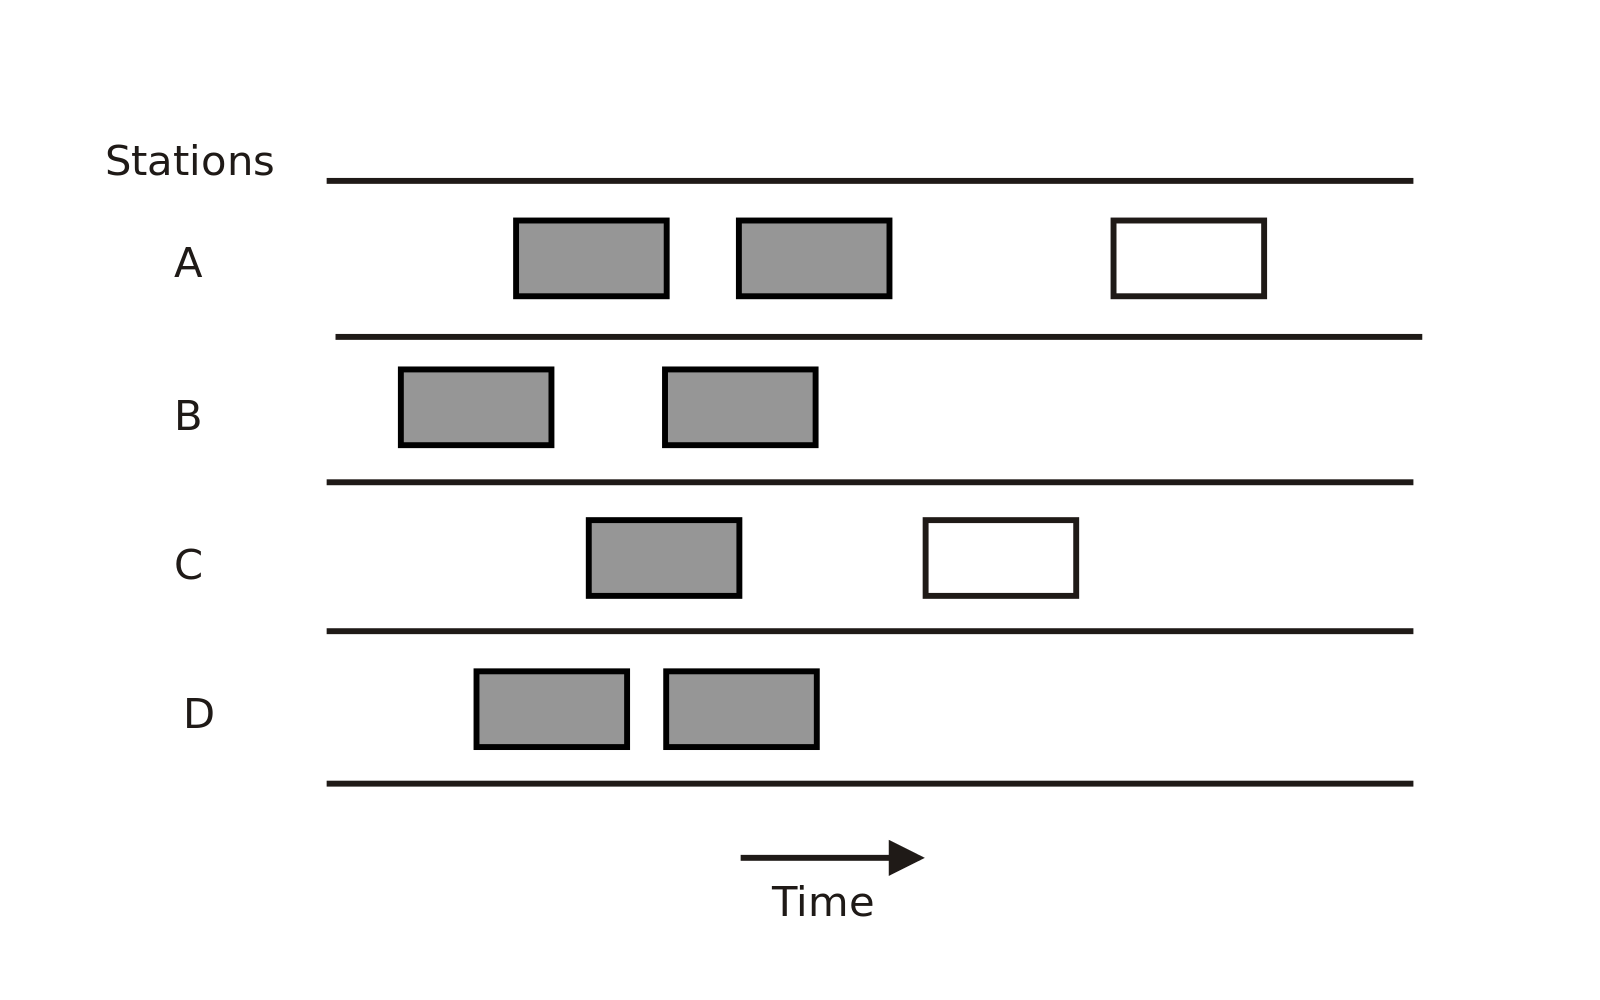
\includegraphics[scale=0.15]{pureALOHA.png}\\
  \tiny{Credit: helix89 of Wikipedia}\\
  A visualisation of pure ALOHA\\
  Shaded slots indicate collision
\end{center}

\filbreak
\textbf{Slotted ALOHA}:

Unlike pure ALOHA, where packets were sent continuously, slotted ALOHA creates discrete timeslots for packets to be sent. This reduces the chance of packets overlapping and ruining the transmission of each packet in that case. This means the probability of a successful transmission is $G\times e^{-G}$, greater than that of pure ALOHA.

\begin{center}
  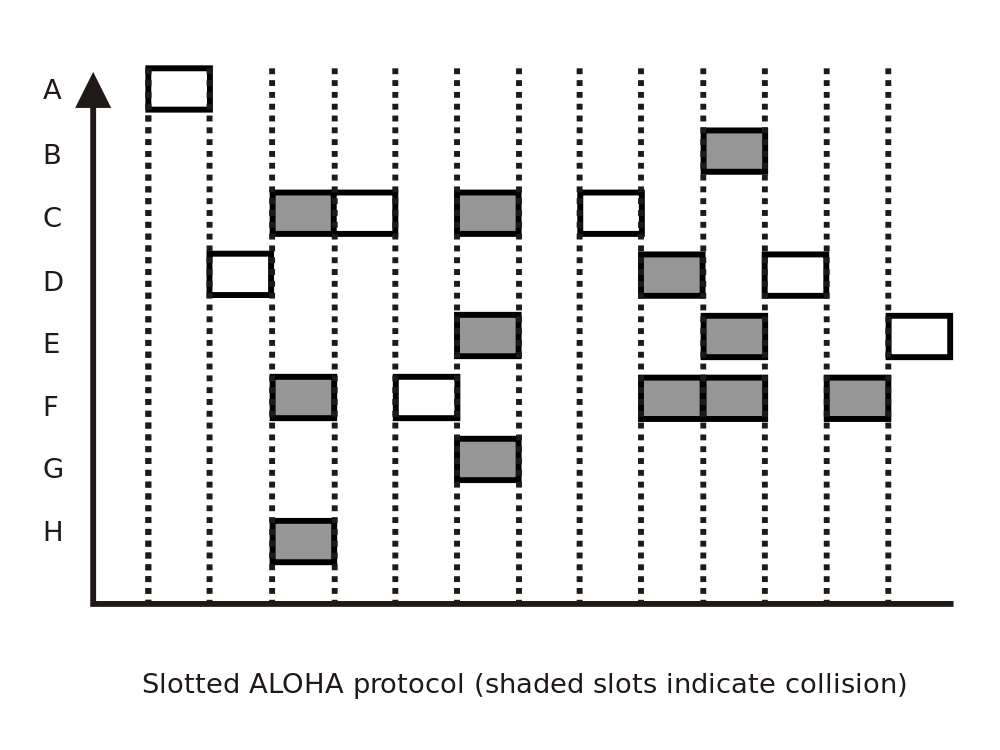
\includegraphics[scale=0.2]{slottedALOHA}\\
   \tiny{Credit: helix89 of Wikipedia}\\
\end{center}

\subsubsection{CSMA: Carrier Sense Multiple Access}

\textbf{Random Access}

This protocol ensures that a node checks if the network medium is idle before it transmits data.

CSMA can also be extended with collision detection, which is denoted as \textbf{CSMA/CD}.

This protocol, whilst transmitting, keeps listening for other nodes transmitting at the same time. If this is detected, it will stop transmitting the data and begin transmitting a \textit{jam signal}. This signal alerts the receiver that a collision has occurred. 

It will wait the minimum amount of time that it will take for the receiver to receive the jam signal, and it will then try to retransmit. If this keeps occurring, it will approach the maximum number of retransmissions. When reached, the transmission attempts will be aborted. It will then start from the beginning, waiting to see if anything else is transmitting before it makes another attempt.

\subsubsection{'Taking Turns'}

\textbf{Token Passing}

This method waits for a token to be passed between nodes, authorising them to communicate. The benefit is it prevents collisions from occurring and maximum throughput can be obtained when demand is heavy, albeit with a latency overhead to set-up the transfer. The downside is the latency issue, which would occur when demand is light.

\textbf{Polling}

When a device wishes to transmit, it will poll the manager of the networking medium if it is okay to transmit to some other node.

\subsection{Switch Self-Learning}

When a frame is received, the switch will learn which host can be reached through which network interface. This information is stored in the \textit{switch table}. This table will gradually be populated over time.

\subsection{CRC: Cyclic Redundancy Check}

Error-detecting code used by Ethernet and other mediums. Common as its simple to implement at the hardware level. 'CRC' is usually followed by a number, e.g. 'CRC-4', which means that we would be performing the calculation:

\[
\frac{\text{Sequence of bits we want to send}}{\text{Sequence of 4 bits}}
\]

The sequence will usually be provided to you in an exam, and can be called \textbf{generators}.

\newpage
\large\textbf{CRC for Dummies}

Bitstream we want to send: \texttt{1010111001}\\
Generator: \texttt{1001}

For example, let's say we have a sequence of 10 bytes that we want to send, and will be obtaining error-detection via CRC-4.

\textbf{Step 1}:

Take the length of the generator, and subtract one.

\[ |1001| - 1  = 3\]

We pad the bitstream with this number of zeroes, from the right.

So now, we have: \texttt{1010111001 000}

\textbf{Step 2}:

Now we shall take the padded bitstream and binary divide it by the generator.

\textbf{The aim} is to find the remainder, and append it to the message to be sent. This is because when the message
is received on the other end, it will divide cleanly with no remainder. If there is a remainder found on the receiving end, it means that a transmission error has occurred and the bitstream will need to be sent again.

This is how we divide the bitstream by the generator:

\begin{lstlisting}
      _______________
1001 | 1010111001 000        # start of divison
       1001|||||| |||        # XOR 4 leftmost bits with the generator
       ----vv|||| |||         
         1111|||| |||        # if remainder is zero, we ignore the result
         1001|||| |||          and then XOR the next four bits with the 
         ----v||| |||          first bit equal to one
          1101||| |||
          1001||| |||
          ----v|| |||
           1000|| |||
           1001|| |||
           ----vv v||
              101 0||
              100 1||
              -----vv
                1 100        # notice how the original bitstream
                1 001          is now equal to zero
                -----        # we stop here, and the number 
                  101          we have left is our remainder.
\end{lstlisting}
\filbreak
\textbf{Step 3}:

Now we have the \textbf{remainder}. We append this to the \textbf{original bitstream}, such that:

\texttt{1010111001 101} will be sent.

You can check that this is correct by dividing the message that is sent by the generator.

\begin{lstlisting}
      _______________
1001 | 1010111001 101
       1001|||||| |||
       ----vv|||| |||
         1111|||| |||
         1001|||| |||
         ----v||| |||
          1101||| |||
          1001||| |||
          ----v|| |||
           1000|| |||
           1001|| |||
           ----vv v||
              101 1||
              100 1||
              -----vv
                1 001
                1 001
                -----
                    0    # remainder is equal to zero!
\end{lstlisting}

As the remainder is equal to zero, the message has been sent without error!

\subsection{Switches versus Routers}

\begin{center}
  \definecolor{light-gray}{gray}{0.95}
  \definecolor{heavy-gray}{gray}{0.80}
  \rowcolors{1}{light-gray}{heavy-gray}
  \begin{tabular}{|p{1.8cm}|p{4cm}|p{4cm}|}
    \rowcolor{white}\hline
    & \textbf{Router} & \textbf{Switch}\\
    \hline\hline
    Used For & Connecting  $>= 2$ networks & Connecting $>= 2$ nodes usually in the same network\\
    \hline
    Used In & LANs, WANs & LANs\\
    \hline
    NAT & \checkmark & \\
    \hline
    DHCP & \checkmark & \\
    \hline
    Addressing & IPs & MACs\\
    \hline
    Bandwidth Sharing & Dynamic (can change bandwidth available at each port) or Static & Static\\
    \hline
    
  \end{tabular}
\end{center}

\subsection{MAC: Media Access Control}

A \textbf{MAC Address} is a \textit{unique identifier assigned to network interfaces} to allow communication within the physical layer of the OSI model. For example, in one laptop, a MAC Address will be assigned to both its \textit{wireless networking card} and its \textit{Ethernet networking card} within their respective ROMs.

A MAC Address is most commonly 6 bytes, but newer versions are 8. They in 6 or 8 groups (depending on the address length) of two hexadecimal characters. The first half denotes the manufacturer, whereas the second half denotes the specific hardware.

In addition to the MAC Address found in the hardware, a local network administrator can create a MAC Address for the network interface, where all bytes represent the specific network interface.

\subsubsection{ARP: Address Resolution Protocol}

Used for mapping an IP address to a MAC address, and is only used \textit{within a sole network}, never between two or more different networks.

Initially, a query will be sent to each device in a network requesting that a device with a certain IP address, e.g. 192.168.1.5, reply to it. The corresponding device will respond with its MAC address. This result is cached in a lookup table. Consequently, a device may use its lookup table instead of sending a query to the entire network the next time a device's MAC address is required.

\end{document}